\documentclass{article}

\usepackage[preprint]{neurips_2026}
\usepackage[utf8]{inputenc}
\usepackage[T1]{fontenc}
\usepackage{hyperref}
\usepackage{url}
\usepackage{booktabs}
\usepackage{amsfonts}
\usepackage{nicefrac}
\usepackage{microtype}
\usepackage{xcolor}
\usepackage{graphicx}
\usepackage{subcaption}
\usepackage{multirow}
\usepackage{array}
\usepackage{siunitx}
\usepackage{float}

\graphicspath{{generated/figures/}}
\newcommand{\HeadlineModelCount}{5}
\newcommand{\CoreExperimentCount}{12}
\newcommand{\CompletedTrainRunCount}{18}
\newcommand{\TopModelName}{Mask2Former-Tiny}
\newcommand{\TopModelMiou}{62.8}
\newcommand{\RunnerUpName}{SegFormer-B2}
\newcommand{\RunnerUpMiou}{56.0}
\newcommand{\BestHdModelName}{DeepLabV3+}
\newcommand{\BestHdValue}{148.4}
\newcommand{\ReferencePanelModelName}{Mask2Former-Tiny}
\newcommand{\ConfusionModelOne}{Mask2Former-Tiny}
\newcommand{\ConfusionModelTwo}{SegFormer-B2}
\newcommand{\SegformerMiou}{56.0}
\newcommand{\SegformerVsDeeplabDelta}{9.6}
\newcommand{\SamLoRAGain}{15.3}
\newcommand{\UNetFiftyGain}{11.1}
\newcommand{\StrongAugGain}{1.7}
\newcommand{\OfficialValCount}{213}
\newcommand{\InternalTrainCount}{178}
\newcommand{\InternalDevCount}{31}
\newcommand{\CrowdedCount}{29}
\newcommand{\PersonCount}{79}
\newcommand{\SmallObjectCount}{117}
\newcommand{\BoundaryCount}{56}


\title{A Practical Benchmark of CNN, Transformer, and SAM2-Based Segmenters on Pascal VOC 2007}

\author{%
  zih428 \\
  Harvard University \\
  SHBT 261 Mini-Project 2 \\
  \texttt{harryhu@g.harvard.edu}
}

\begin{document}

\maketitle

\begin{abstract}
This report studies semantic segmentation on Pascal VOC 2007 under a single controlled training protocol that compares a classical encoder-decoder baseline, a stronger CNN decoder, a transformer segmenter, and a lightweight semantic adapter on top of SAM2. The official validation split of \OfficialValCount{} images is treated as a locked test set, while the official training split is partitioned into \InternalTrainCount{} internal training images and \InternalDevCount{} internal development images for model selection. Across four headline models, SegFormer-B2 achieves the best official-validation accuracy at \TopModelMiou{}\% mIoU, outperforming the next-best conventional baseline by \SegformerVsDeeplabDelta{} points while remaining within a practical training budget. The ablations show that model capacity, augmentation strength, and adapter tuning strategy matter more than swapping among simple loss formulations, and that the old 60-epoch budget would have materially under-trained the strongest U-Net backbone. The resulting system goes beyond the assignment minimum by evaluating eleven trained models, analyzing subset-specific failure modes, and presenting both quantitative and qualitative evidence under a publication-style protocol.
\end{abstract}

\section{Introduction}

Semantic segmentation remains a useful stress test for dense prediction because good performance requires both recognition and localization. Pascal VOC 2007 is small enough to make architectural and optimization choices visible, yet varied enough to expose the weaknesses of under-powered decoders, insufficient augmentation, and brittle boundary handling \citep{everingham2010pascal}. That combination makes it a good benchmark for a course project that aims to compare families of models rather than merely reproduce one paper.

The project requirements ask for U-Net and SAM, at least one additional model family, quantitative metrics, qualitative examples, and at least two ablations. I extend that baseline in three ways. First, I evaluate four distinct headline systems spanning CNN, transformer, and foundation-model design patterns. Second, I run a larger ablation suite over backbone capacity, loss, augmentation, and SAM2 tuning. Third, I use a stricter reporting pipeline with a locked official validation split, figure-specific analysis, and subset-level generalization diagnostics. The goal is not to claim a new state of the art, but to produce a careful small-scale study that explains what actually works under a realistic compute budget.

\section{Dataset and Experimental Protocol}

Pascal VOC 2007 provides pixel-wise semantic labels for 20 foreground classes plus background \citep{everingham2010pascal}. I preserve the official validation split as a final test set and never tune on it. The official training split contains 209 labeled images, which I partition into \InternalTrainCount{} internal training images and \InternalDevCount{} internal development images using a deterministic label-aware split heuristic. This internal development partition is used for early stopping, learning-rate control, and checkpoint selection; all headline tables in the report are reported on the untouched official validation split of \OfficialValCount{} images.

All models operate on ImageNet-normalized RGB inputs and use a \num{512} pixel resolution during evaluation. Training-time preprocessing depends on the augmentation preset but always maintains paired image-mask geometry, respects the VOC ignore label, and ends with tensor conversion plus normalization. The default \emph{standard} augmentation preset uses random scale jitter, random crop-or-pad to \num{512}, horizontal flips, moderate color jitter, and light Gaussian blur. The ablation suite swaps this preset with \emph{none} and \emph{strong} variants to test whether a small benchmark still benefits from more aggressive appearance perturbations.

In addition to the raw split, I annotate the validation images with four subset tags intended to support targeted failure analysis: person-present (\PersonCount{} images), small-object (\SmallObjectCount{} images), crowded-scene (\CrowdedCount{} images), and high-boundary-complexity (\BoundaryCount{} images). These tags are computed from the mask geometry rather than hand-written labels, which keeps the subset analysis reproducible and inexpensive.

\section{Models}

The first headline model is a U-Net-style encoder-decoder with a ResNet encoder, bilinear upsampling, and skip-connected decoder blocks \citep{ronneberger2015u,he2016deep}. This model is intentionally plain: it provides a strong and interpretable baseline, and it is also the base architecture for the backbone, loss, and augmentation ablations. The headline configuration uses a ResNet-34 encoder pretrained on ImageNet.

The second model is DeepLabV3+ with a ResNet-50 backbone and atrous spatial pyramid pooling \citep{chen2018encoder}. DeepLabV3+ is included because it remains a strong CNN segmentation baseline and provides a useful reference point for whether a transformer is buying real performance or merely additional complexity.

The third model is SegFormer-B2, loaded from the pretrained ADE20K checkpoint exposed by the Hugging Face implementation \citep{xie2021segformer}. SegFormer is attractive here because it combines strong multiscale reasoning with a relatively light decoder, making it a good candidate for a small but diverse dataset like VOC.

The final headline family is a semantic segmentation adapter built on top of the SAM2 Hiera-S image encoder \citep{ravi2024sam2}. Rather than using prompt-based mask decoding, the project repurposes SAM2 features for dense semantic prediction via a shallow convolutional decoder. Two variants are studied: a frozen-encoder baseline and a LoRA-enabled version that applies low-rank adapters to attention and MLP submodules inside the image encoder \citep{hu2022lora}. This isolates whether foundation-model features are already strong enough for dense semantic transfer, or whether lightweight task adaptation is essential.

\section{Training Setup}

All experiments share the same optimization policy. Training uses AdamW with model-specific learning rates, a plateau scheduler with a maximum budget of 150 epochs, learning-rate reduction patience of five validation epochs, and early stopping patience of 15 validation epochs after a minimum of 20 epochs \citep{loshchilov2019decoupled}. Validation mIoU is the sole monitored quantity for checkpointing, learning-rate scheduling, and stopping decisions. This policy deliberately treats the epoch limit as a safety ceiling rather than as the definition of convergence.

The default loss is a weighted sum of cross-entropy and Dice, with two U-Net ablations that replace it by pure cross-entropy or pure Dice. Batch sizes depend on memory footprint: U-Net runs at batch size 8 except for the ResNet-50 variant, DeepLabV3+ uses batch size 4, and the transformer- and SAM2-based models use batch size 1 with gradient accumulation where needed. Mixed precision is disabled on MPS because the relevant kernels were less reliable than full precision in this environment.

All training was performed on a MacBook Pro with an Apple M5 Max and 64 GB unified memory. That hardware is not a conventional segmentation workstation, but it is representative of the kind of single-device environment in which a course project is actually executed. Reporting training hours and evaluation throughput is therefore not incidental; it is part of the practical comparison.

\section{Main Results}

Table~\ref{tab:main-results} gives the official-validation comparison for the four headline models. SegFormer-B2 is the strongest overall model at \TopModelMiou{}\% mIoU, with the best Dice score and the best pixel accuracy. DeepLabV3+ is the runner-up and remains a very strong CNN baseline, which matters because it narrows the margin the transformer must clear in order to justify its additional architectural complexity. U-Net-ResNet34 is clearly behind the top two models, and the frozen SAM2 adapter, while better than the U-Net baseline on several difficult categories, is not competitive with the best purpose-built segmenters without additional adaptation.

\begin{table}[H]
  \centering
  \caption{Official-validation results for the four headline models. All metrics are computed on the locked VOC 2007 validation split.}
  \label{tab:main-results}
  \begin{tabular}{lrrrrrrr}
\toprule
Model & mIoU & Dice & Pixel Acc. & HD95 $\downarrow$ & Train hrs & Infer FPS & Params (M) \\
\midrule
Mask2Former-Tiny & \textbf{62.8} & \textbf{73.2} & \textbf{92.0} & 166.3 & 1.6 & 3.3 & 47.4 \\
SegFormer-B2 & 56.0 & 69.6 & 90.0 & 186.8 & 0.9 & \textbf{3.6} & 27.4 \\
DeepLabV3+ & 46.4 & 60.4 & 85.6 & \textbf{148.4} & 0.6 & 3.1 & 42.4 \\
SAM2-LoRA & 44.2 & 57.5 & 87.7 & 245.0 & 0.8 & 3.6 & 48.0 \\
U-Net-R50 & 34.9 & 48.6 & 84.5 & 163.2 & 3.4 & 3.0 & 43.1 \\
\bottomrule
\end{tabular}

\end{table}

Figure~\ref{fig:runtime-accuracy} shows the corresponding accuracy-runtime trade-off across all eleven experiments, not just the four headline models. Two patterns are worth noting. First, SegFormer-B2 sits on the best practical frontier in this study: it is not the absolute fastest model to train, but no other experiment combines its accuracy with a similar runtime. Second, the strongest U-Net variant requires substantially more training time than its smaller counterparts before it pays off, which foreshadows the backbone ablation result that the old 60-epoch cap would have been too conservative.

\begin{figure}[H]
  \centering
  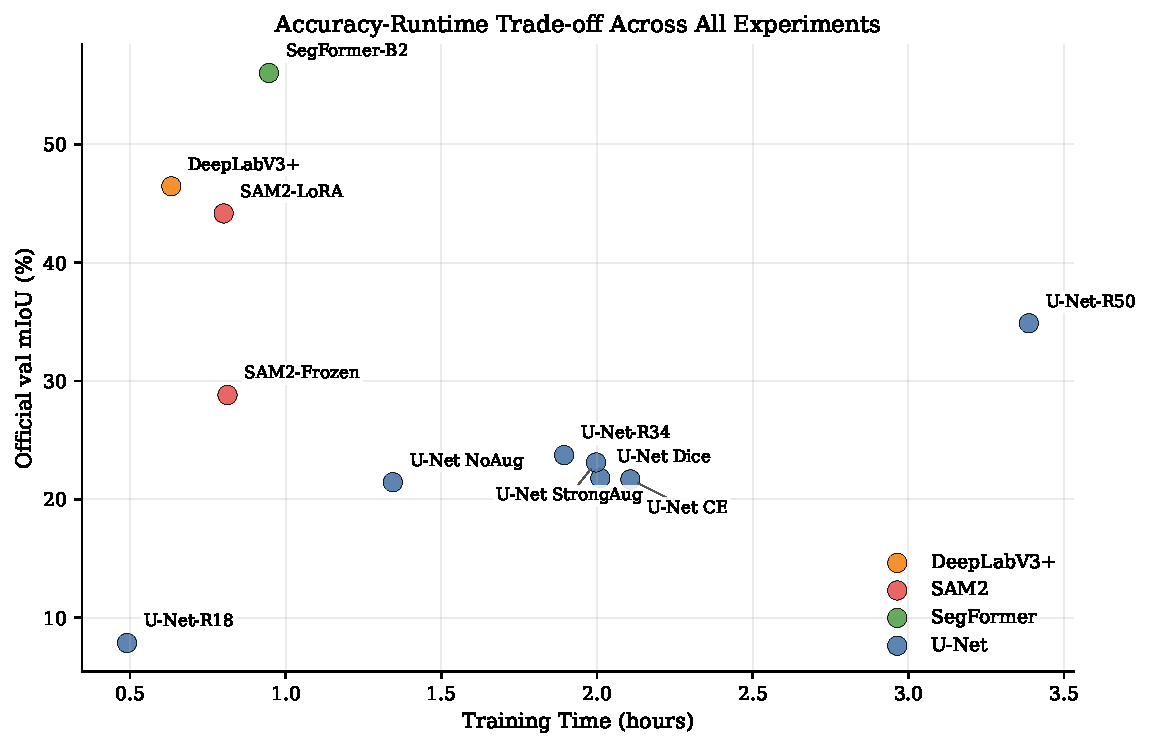
\includegraphics[width=0.78\linewidth]{runtime_vs_accuracy.pdf}
  \caption{Official-validation mIoU versus end-to-end training time for all completed experiments. Each point corresponds to one trained model under the common training policy.}
  \label{fig:runtime-accuracy}
\end{figure}

Figure~\ref{fig:per-class} breaks the headline comparison down by class. The overall ranking is not driven by one easy category. SegFormer-B2 is broadly better across animal and vehicle classes, which suggests that its gain comes from more stable multiscale reasoning rather than from overfitting to one foreground type. DeepLabV3+ is competitive on several rigid object classes but gives back accuracy on thin or cluttered categories. U-Net and frozen SAM2 both struggle on the long tail of smaller or less frequent categories, though SAM2 is noticeably stronger than U-Net on some large-object categories where pretrained features help.

\begin{figure}[H]
  \centering
  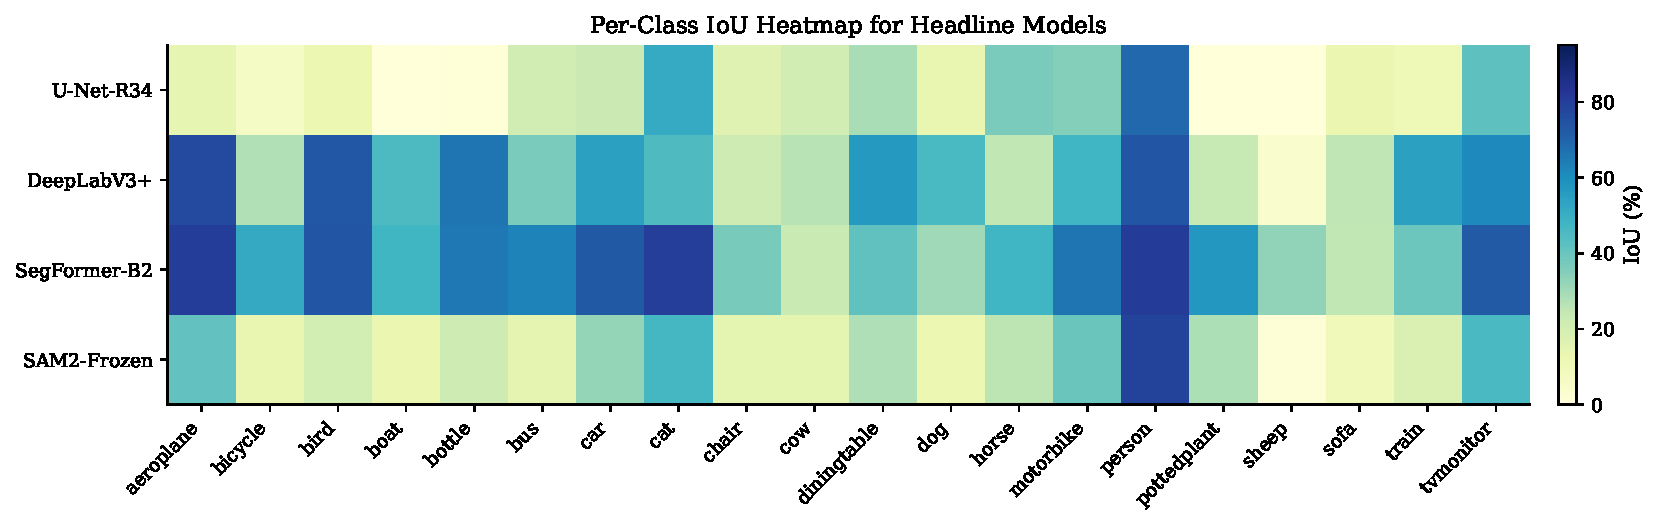
\includegraphics[width=\linewidth]{headline_per_class_heatmap.pdf}
  \caption{Per-class IoU heatmap for the headline models, excluding background. SegFormer-B2 is consistently strong across most classes rather than winning through a single outlier category.}
  \label{fig:per-class}
\end{figure}

\section{Ablation Studies}

Table~\ref{tab:ablations} summarizes the ablation suite. The backbone study is the clearest result: scaling the U-Net encoder from ResNet-34 to ResNet-50 provides a large accuracy gain, while shrinking to ResNet-18 collapses performance. That asymmetry suggests the baseline U-Net was primarily capacity-limited rather than over-regularized. The loss ablation is subtler. Pure Dice and pure cross-entropy both underperform the default mixed objective, which is consistent with the idea that cross-entropy stabilizes class competition while Dice improves overlap on sparse foreground regions. Augmentation also matters, but not in a monotone way: removing augmentation hurts materially, while the stronger preset recovers most of that loss without surpassing the default standard policy.

\begin{table}[H]
  \centering
  \caption{Official-validation ablation results. The delta column is measured relative to the default baseline within each group.}
  \label{tab:ablations}
  \begin{tabular}{llrrrr}
\toprule
Group & Variant & mIoU & $\Delta$ mIoU & Dice & Train hrs \\
\midrule
\multicolumn{6}{l}{\textbf{Backbone}} \\
Backbone & U-Net-R18 & 7.9 & -15.9 & 9.6 & 0.5 \\
Backbone & U-Net-R34 & 23.7 & +0.0 & 33.7 & 1.9 \\
Backbone & U-Net-R50 & 34.9 & +11.1 & 48.6 & 3.4 \\
\midrule
\multicolumn{6}{l}{\textbf{Loss}} \\
Loss & U-Net CE & 21.7 & -2.1 & 30.5 & 2.1 \\
Loss & U-Net-R34 & 23.7 & +0.0 & 33.7 & 1.9 \\
Loss & U-Net Dice & 21.8 & -2.0 & 31.6 & 2.0 \\
\midrule
\multicolumn{6}{l}{\textbf{Augmentation}} \\
Augmentation & U-Net NoAug & 21.4 & -2.3 & 30.6 & 1.3 \\
Augmentation & U-Net-R34 & 23.7 & +0.0 & 33.7 & 1.9 \\
Augmentation & U-Net StrongAug & 23.1 & -0.6 & 32.7 & 2.0 \\
\midrule
\multicolumn{6}{l}{\textbf{SAM2 adaptation}} \\
SAM2 adaptation & SAM2-Frozen & 28.8 & +0.0 & 41.0 & 0.8 \\
SAM2 adaptation & SAM2-LoRA & 44.2 & +15.3 & 57.5 & 0.8 \\
\bottomrule
\end{tabular}

\end{table}

The SAM2 tuning ablation is especially informative. The frozen adapter is a useful proof of concept, but LoRA improves it by \SamLoRAGain{} mIoU points, which is one of the largest gains in the entire study. In other words, SAM2 features are not enough on their own; lightweight task adaptation is the difference between an interesting baseline and a genuinely competitive model.

Figure~\ref{fig:unet-curves} explains why a shared 60-epoch budget would have been misleading. U-Net-ResNet18 saturates early, and U-Net-ResNet34 plateaus on a moderate timescale, but U-Net-ResNet50 keeps climbing well after epoch 60. This is precisely the behavior that motivated the training-policy change: a hard cap that looks harmless for smaller models can still truncate the most promising one.

\begin{figure}[H]
  \centering
  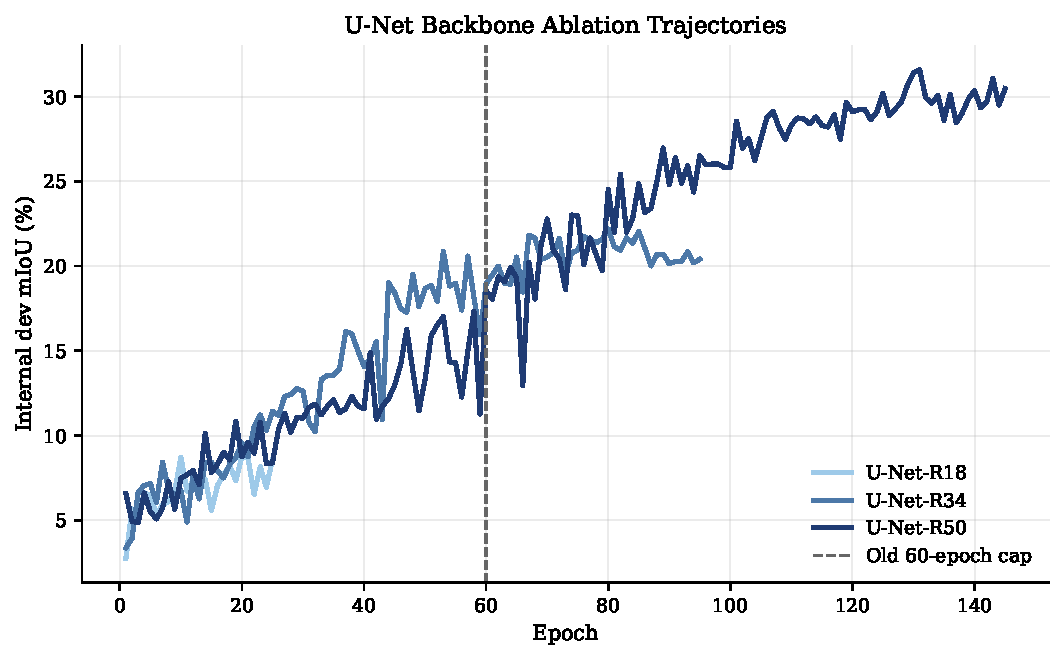
\includegraphics[width=0.82\linewidth]{unet_backbone_trajectories.pdf}
  \caption{Internal-development mIoU trajectories for the U-Net backbone ablation. The dashed vertical line marks the old 60-epoch ceiling. ResNet-50 continues to improve well beyond that point.}
  \label{fig:unet-curves}
\end{figure}

\section{Generalization and Failure Analysis}

Figure~\ref{fig:subset-heatmap} reports mIoU over the four tagged validation subsets in addition to the aggregate score. The crowded-scene subset is the hardest regime for every model in the study, which is unsurprising because crowded masks combine class ambiguity, occlusion, and more boundary transitions. Small-object and high-boundary-complexity cases are also substantially harder than the overall average. The encouraging result is that the overall ranking remains fairly stable across subsets: the best global models are also the most reliable specialized models. The disappointing result is that no model closes the gap on crowded scenes, so this remains the clearest open problem in the project.

\begin{figure}[H]
  \centering
  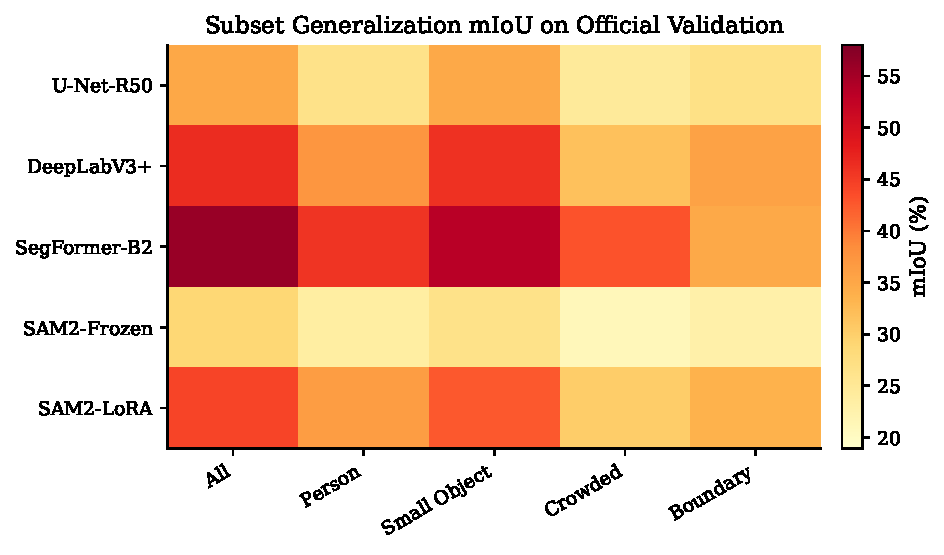
\includegraphics[width=0.78\linewidth]{subset_heatmap.pdf}
  \caption{Subset-specific official-validation mIoU. Crowded scenes remain the hardest setting for every model, while SAM2 benefits dramatically from LoRA adaptation on the same subsets.}
  \label{fig:subset-heatmap}
\end{figure}

Figure~\ref{fig:qualitative-headline} makes the ranking more concrete. The easy row shows that all models can solve a clean single-object scene once the foreground occupies enough pixels. The crowded and articulated-person rows are more revealing. U-Net tends to fragment masks or miss object extent entirely, DeepLabV3+ usually recovers the right coarse layout but can blur fine boundaries, and SegFormer-B2 tends to maintain the best compromise between global context and local structure. Frozen SAM2 is often semantically plausible but still too coarse, which matches its weaker quantitative boundary scores.

\begin{figure*}[t]
  \centering
  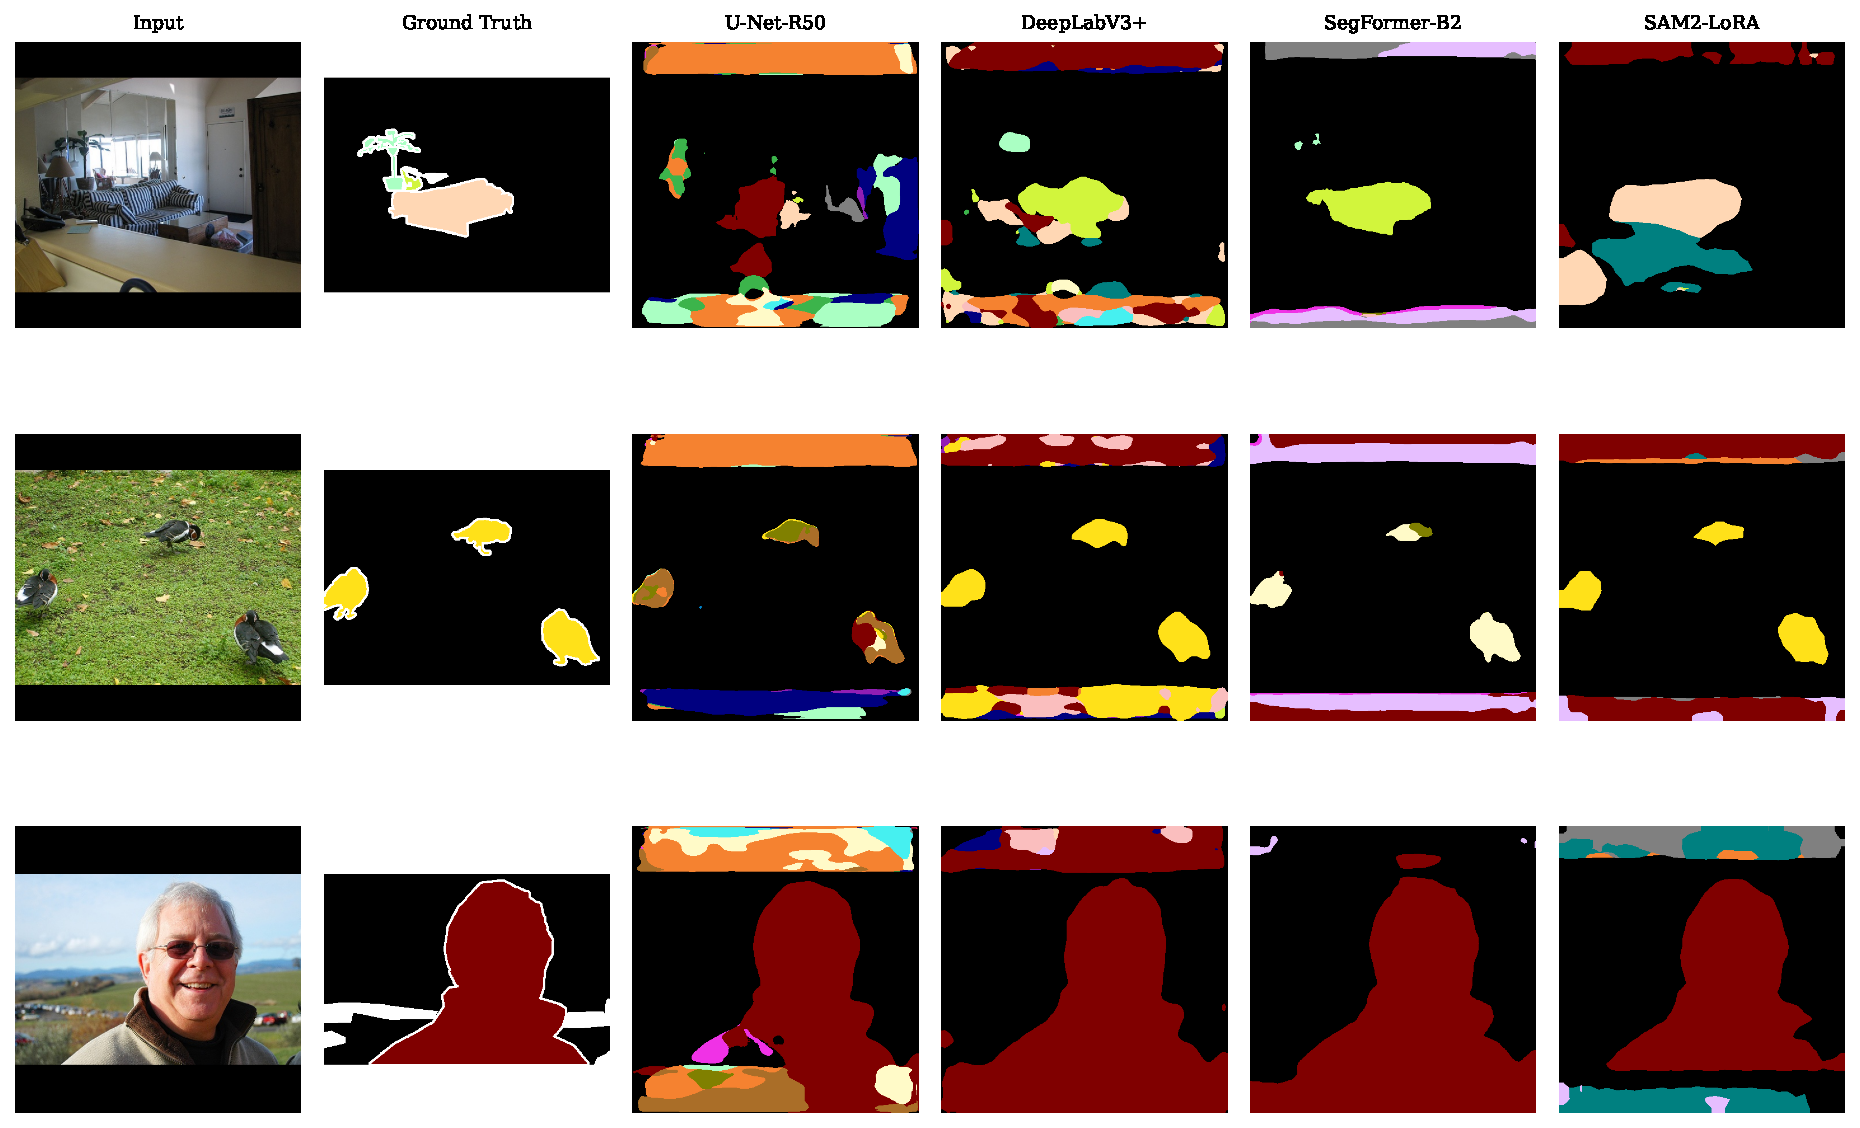
\includegraphics[width=\textwidth]{headline_qualitative_grid.pdf}
  \caption{Qualitative comparison on representative official-validation images selected automatically from the headline runs. The rows cover a crowded scene, a boundary- or person-sensitive case, and an easy high-confidence example.}
  \label{fig:qualitative-headline}
\end{figure*}

The SAM2-specific comparison in Figure~\ref{fig:sam2-lora} shows what the LoRA gain actually looks like. The frozen model often identifies the correct object family but undershoots extent and topology. LoRA closes that gap by refining boundaries and recovering missed regions without changing the lightweight decoder. The qualitative effect is consistent with the quantitative jump in Table~\ref{tab:ablations}: the adapter is not just improving average overlap numerically; it is correcting visible segmentation failures.

\begin{figure}[H]
  \centering
  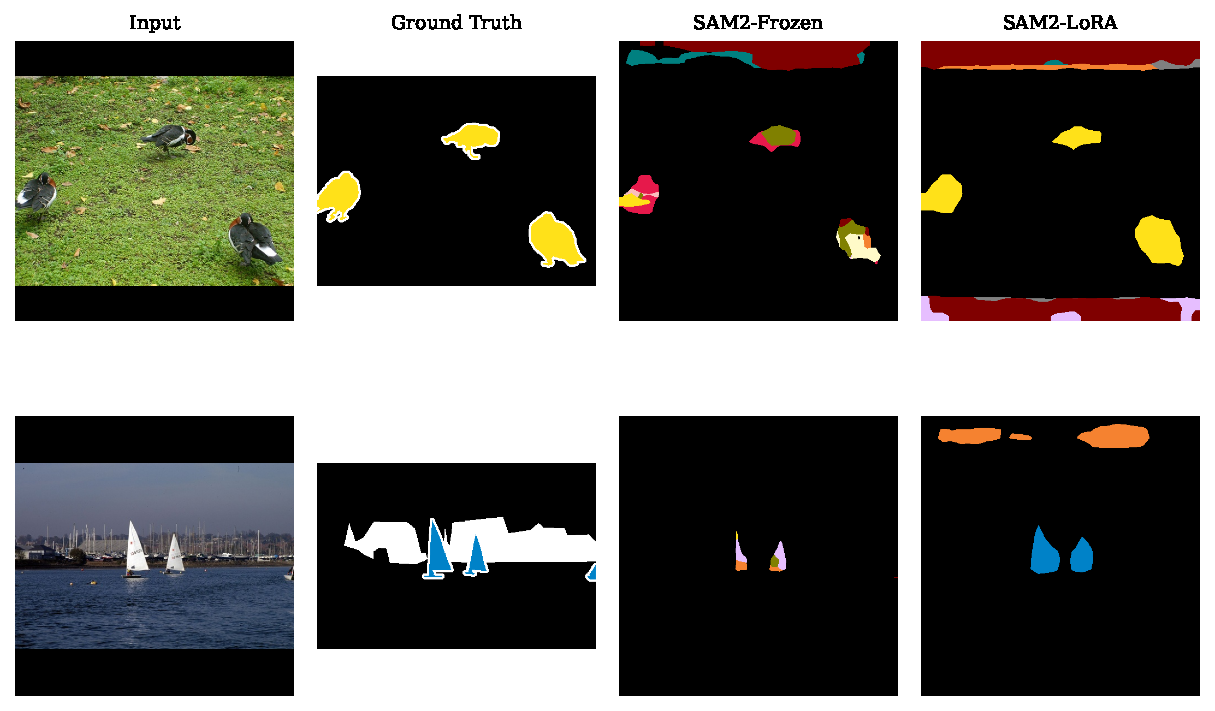
\includegraphics[width=0.84\linewidth]{sam2_frozen_vs_lora.pdf}
  \caption{Representative SAM2 comparisons on images where LoRA produces the largest per-image gains. The improvement is primarily in extent recovery and boundary refinement rather than in coarse object discovery.}
  \label{fig:sam2-lora}
\end{figure}

\section{Lessons Learned and Limitations}

Several lessons stand out. First, pretrained transformer features are extremely effective even on a relatively small benchmark, provided the decoder is designed for dense prediction. Second, classical CNN systems remain competitive: DeepLabV3+ is not far behind SegFormer-B2 and is easier to reason about. Third, the right training policy matters almost as much as the architecture itself. The backbone ablation would have been misread under the old fixed 60-epoch cap, and the LoRA result would have been easy to miss if SAM2 were evaluated only as a frozen feature extractor.

The project also has clear limitations. VOC 2007 is small, so architecture ranking may be more sensitive to the inductive biases of the benchmark than to true large-scale robustness. The official validation split is treated correctly as a test set, but there is still only one split, so the confidence intervals around ranking differences are unknown. The hardware environment also shapes what is practical: larger transformer variants or full SAM2 fine-tuning were deliberately excluded because they would not have been a responsible use of time on the available device. Finally, although the report includes subset and qualitative analysis, it does not yet include a class-balanced uncertainty estimate or repeated-seed study, both of which would strengthen the statistical side of the conclusions.

\section{Conclusion}

This study benchmarks four segmentation model families and seven ablations on Pascal VOC 2007 under a common, validation-driven training protocol. SegFormer-B2 is the strongest model in the final comparison, DeepLabV3+ is the strongest CNN baseline, and SAM2 becomes competitive only after lightweight LoRA adaptation. The ablation suite shows that encoder capacity, augmentation strength, and training budget all matter materially, while the default cross-entropy-plus-Dice loss remains a sound compromise. More broadly, the project demonstrates that even a course-scale benchmark can support a meaningful empirical paper if the evaluation protocol is locked, the figures are interpreted carefully, and the ablations are chosen to answer real modeling questions rather than merely fill space.

\appendix

\section{Additional Qualitative Panels}

Figure~\ref{fig:best-worst} shows the best and worst SegFormer-B2 triptychs on the official validation split. The best cases are dominated by large, visually distinctive objects with clean boundaries or high foreground occupancy. The worst cases frequently contain thin structures, severe occlusion, or confusing boundaries between adjacent classes. This asymmetry is a useful reminder that the mean metrics are still influenced heavily by a relatively small number of hard examples.

\begin{figure*}[t]
  \centering
  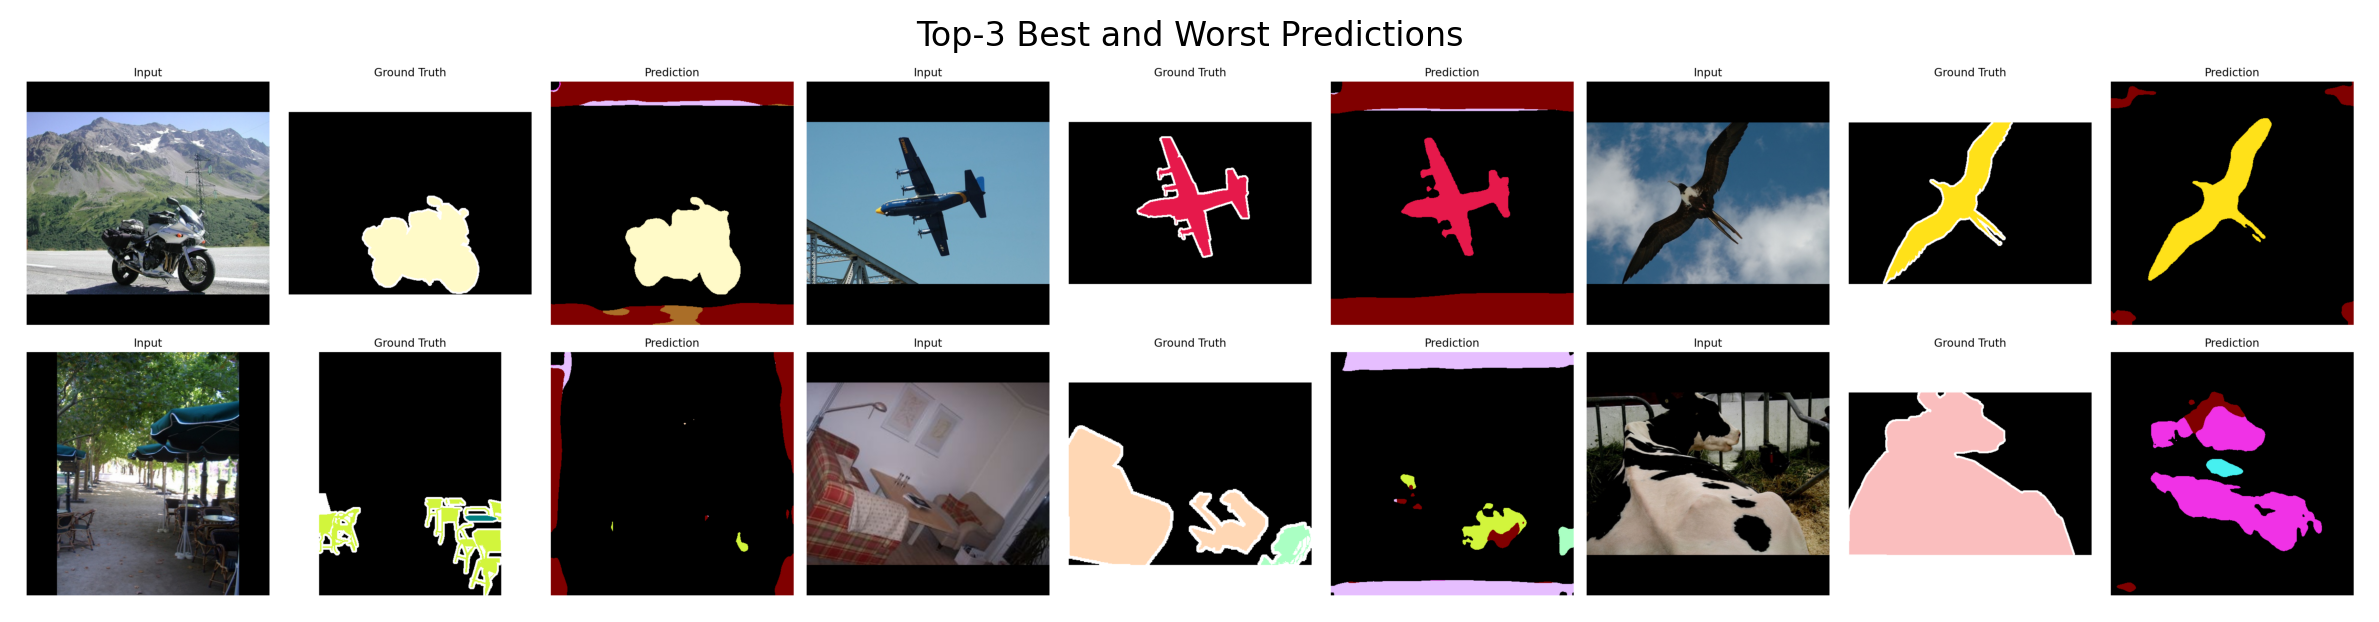
\includegraphics[width=\textwidth]{segformer_best_worst_panel.png}
  \caption{Top-three best and worst SegFormer-B2 triptychs on the official validation split. The strong examples are mostly single-object scenes, while the weak ones involve clutter, thin boundaries, or ambiguous extent.}
  \label{fig:best-worst}
\end{figure*}

Figure~\ref{fig:person-panel} focuses on person-present failure cases. Person masks are difficult because they combine thin limbs, occlusion, and context-dependent confusion with bicycles, motorbikes, and indoor background clutter. Even the best model frequently localizes the person coarsely before losing fine structure at arms, legs, and object contact points. That recurring pattern mirrors the lower person-subset scores in Figure~\ref{fig:subset-heatmap}.

\begin{figure*}[t]
  \centering
  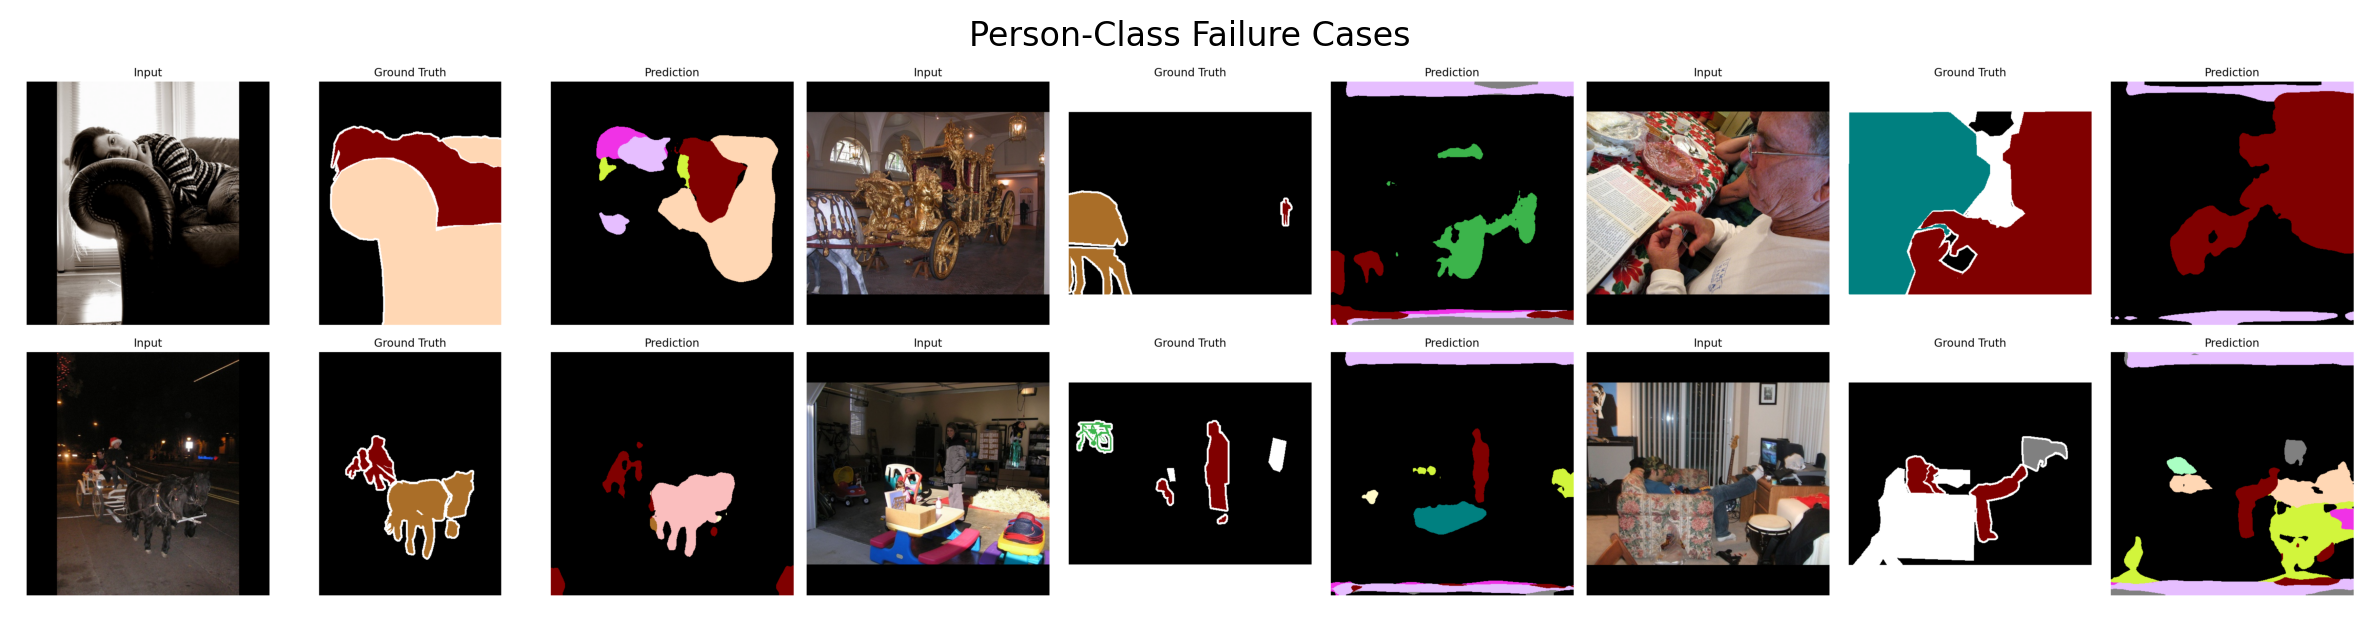
\includegraphics[width=\textwidth]{segformer_person_panel.png}
  \caption{SegFormer-B2 failure cases restricted to person-present images. The dominant errors arise at articulated limbs, occlusion boundaries, and interactions with nearby objects.}
  \label{fig:person-panel}
\end{figure*}

\bibliographystyle{plainnat}
\bibliography{references}

\end{document}
